\mysection{エミッタ接地交流増幅回路の設計}
電流帰還バイアス回路を用いたエミッタ接地交流増幅回路を設計する。この回路が、実際に使用されるエミッタ接地回路である。

\begin{description}
  \setlength{\parskip}{0cm} % 段落間
  \setlength{\itemsep}{0cm} % 項目間
  \item[ゴール] 電流帰還バイアス回路を用いたエミッタ接地交流増幅回路を設計する。
  \item[キーワード] 等価回路、結合キャパシタ$C_1、C_2、C_E$、電圧増幅度、遮断周波数、入力インピーダンス、四端子定数、$V_{BE}-I_E$特性
  \item[ストーリー] エミッタ接地回路の交流成分を考える → 交流等価回路にする → 入力インピーダンス、出力インピーダンスをなんか計算する → 低域遮断周波数、電圧増幅度、結合キャパシタの値を決める。ついでに利得とかも計算する。→ LTspiceで設計 → LTspiceで交流増幅特性(AC解析) → LTspiceで過渡解析 → 計算値と比較
\end{description}

\mysubsection{演習手順}
バイアス設定確認 → 動作点解析 → 交流増幅特性解析の順に行う。
$C_2$ の出力側に次段の入力インピーダンス $R_i = 1$k$\Omega$ を接続することで、中域の増幅度が変化する。
\begin{align}
  & 電圧増幅度(中域) |A_v| = \frac{\beta R'_L}{Z_i} = \frac{R'_L}{Z_i/\beta} \approx \frac{R'_L}{r_e}
  (R'_L = R_L//R_i = \frac{R_LR_i}{R_L+R_i}) \\
  & 電圧利得 20 \log (R'_L/r_e)
\end{align}

\mysubsubsection{過渡解析(中域の増幅度に関して)}
\begin{enumerate}
  \setlength{\parskip}{0cm}
  \setlength{\itemsep}{0cm}  
  \item $v_1 = 10$mV (振幅), 1 kHz
  \item $R_i$ の次段の入力抵抗を1k$\Omega$
  \item $R'_L = R_L // R_i$ より、$R_i$ は、中域の増幅度に影響を与える。
\end{enumerate}
中域増幅度 $|A_v| = \frac{\beta R'_L}{Z_i} = \frac{R'_L}{Z_i/\beta} \approx \frac{R'_L}{r_e}$より、
\begin{align}
  R'_L = R_L // R_i = 818.18 // 10^{3} = 449.999... \fallingdotseq 450[\Omega]\\
  電圧増幅率 |A_v| \approx \frac{R'_L}{r_e} = \frac{450}{4.7272...} = 95.1937... \fallingdotseq 95\\
  電圧利得 20\log(\frac{R'_L}{r_e}) = 20\log(\frac{450}{4.7272...}) = 39.572... \fallingdotseq 39.6\textrm{dB}  
\end{align}

\begin{description}
  \item[課題8] 入力信号 $v_1 =$ 20 mVp-p 1kHz として図\ref{kouryu}の回路を設計し、過渡特性を取得して下さい。 \\
  (用いた回路図とディレクティブを示すこと。図\ref{kouryu}(a)(b))
\end{description}

\begin{figure}[htb]
  \begin{center}
  \subfigure[エミッタ接地交流増幅回路]{	% 副題なし
  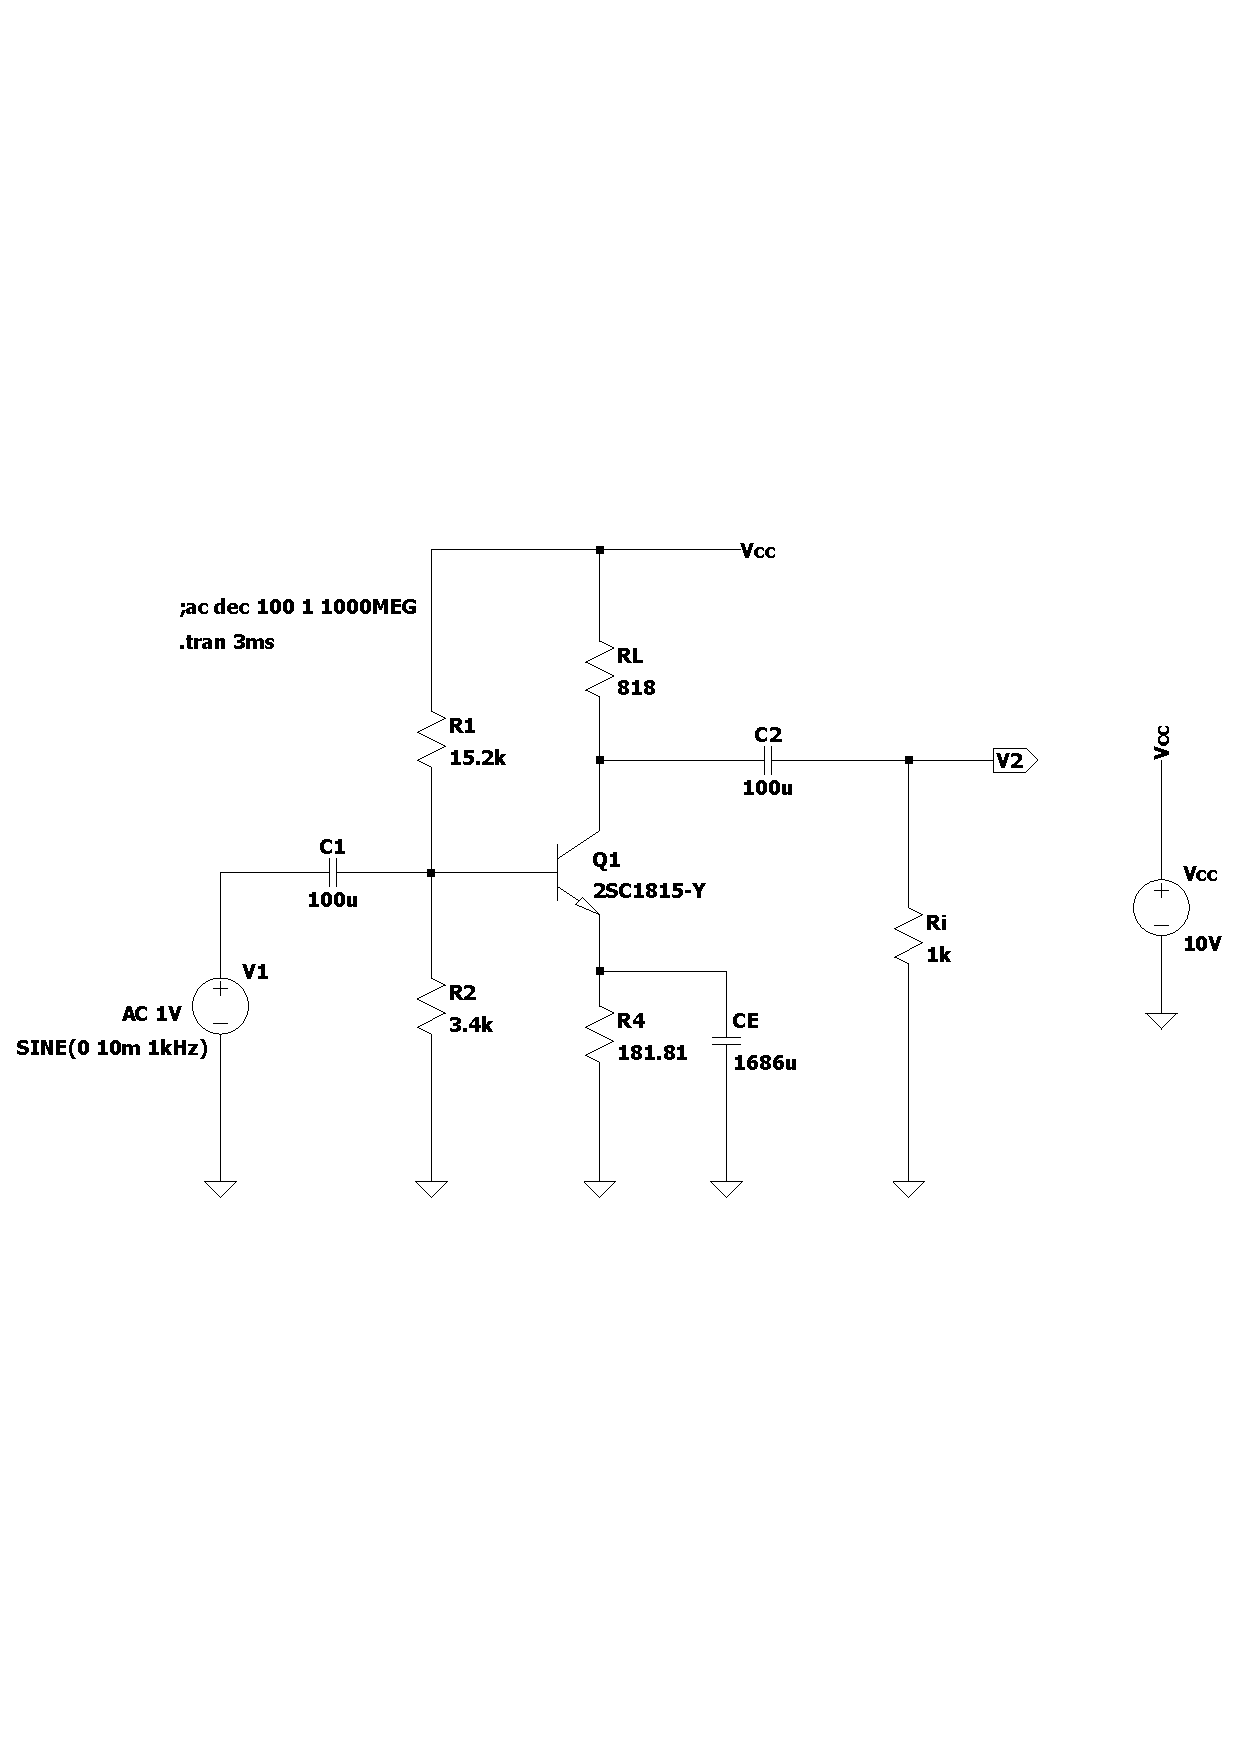
\includegraphics[width=.5\columnwidth]{img/52.pdf}
  }~
  \subfigure[過渡特性結果]{
  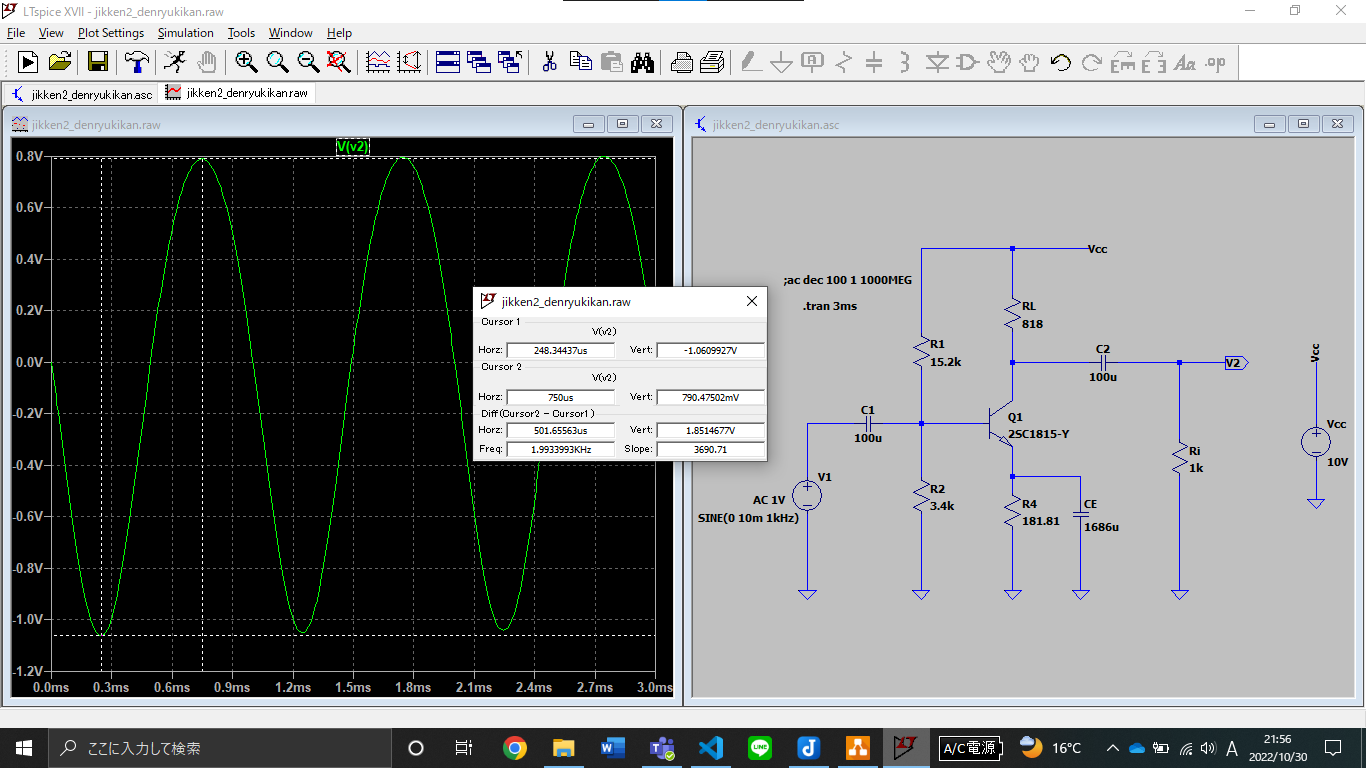
\includegraphics[width=.5\columnwidth]{img/53.png}
  }
  \caption{過渡特性}
  \label{kouryu}
  \end{center}
\end{figure}

\mysubsubsection{AC解析}
\begin{description}
  \item[課題9] 手順に沿って図\ref{ackaiseki}に示すAC解析を行って下さい。\\
「Edit Simulation Command.」→ 「AC解析」→ 「Stop frequency」を"100MEG"に設定 → .ac ディレクティブを回路図に張り付けて「Run」を実行する。
電圧プローブを$v_2$ に設定する。

\begin{figure}[htb]
  \begin{center}
  \subfigure[AC解析結果]{	% 副題なし
  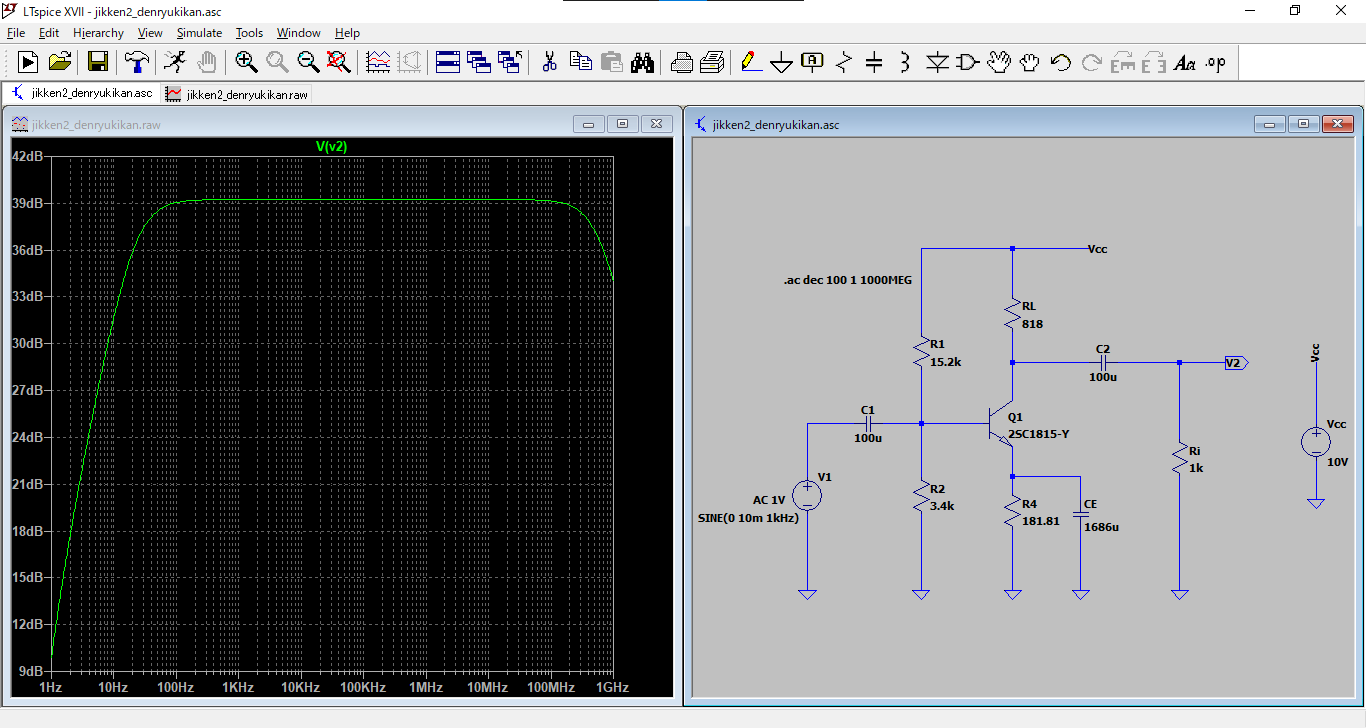
\includegraphics[width=.5\columnwidth]{img/54.png}
  }~
  \subfigure[AC特性(3dB降下をカーソルで取得)]{
  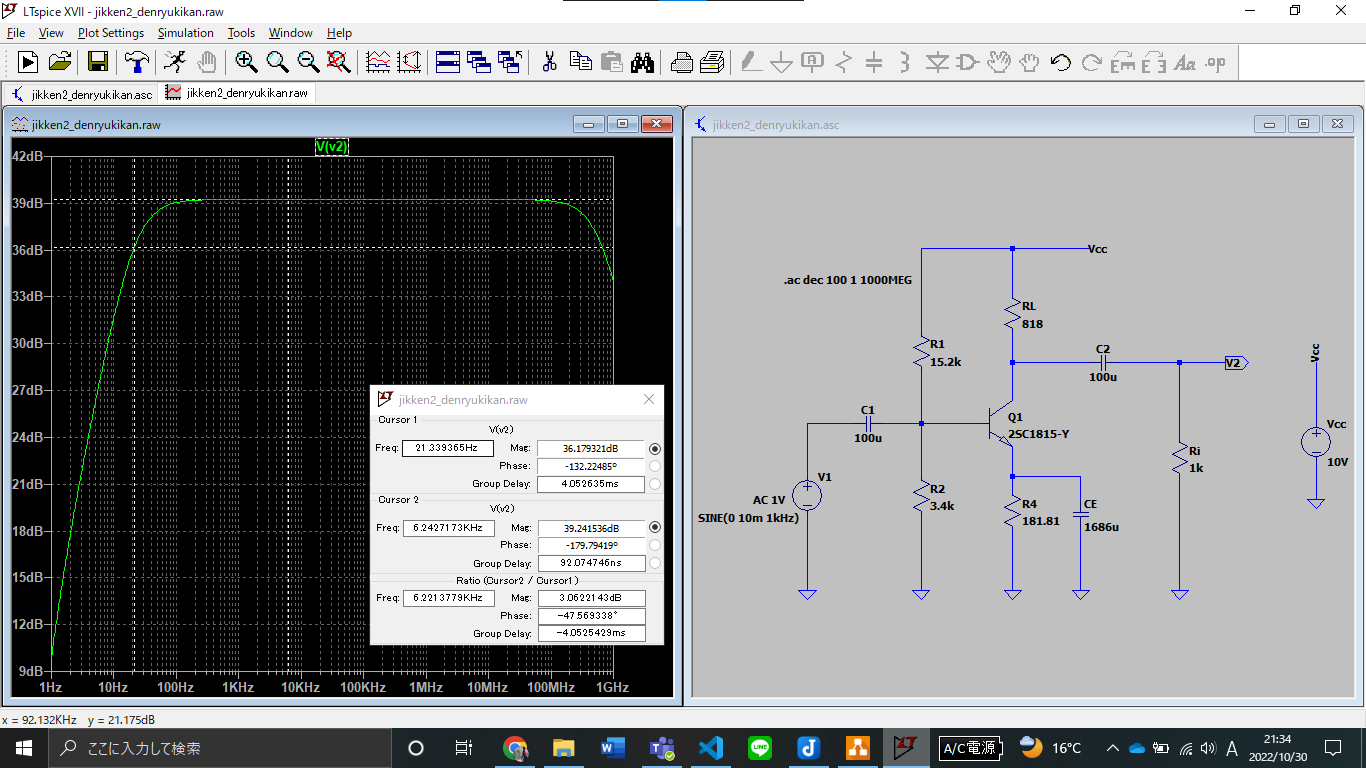
\includegraphics[width=.5\columnwidth]{img/55.png}
  }
  \caption{AC解析}
  \label{ackaiseki}
  \end{center}
\end{figure}

  \item [課題10] 低域遮断周波数、電圧増幅率、電圧利得を計測し、それらの理論値と実測値を比較してください。\\
  低域遮断周波数: 電圧利得が 3dB 降下する周波数\\
  電圧増幅率: 過渡解析において、$v_2$ のp-p 値を求め、$v_2/v_1$ の値を求める。\\
  電圧利得: $20\log|A_v|$ の値をAC解析の中域利得と比較する。

\end{description}